\problemname{Bounty Hunter II}

Spike the bounty hunter is tracking another criminal through space. Luckily for
him hyperspace travel has made the task of visiting several planets a lot
easier. Each planet has a number of Astral Gates; each gate connects with a gate
on another planet. These hyperspace connections are, for obvious safety
reasons, one-way only with one gate being the entry point and the other gate
being the exit point from hyperspace. Furthermore, the network of hyperspace
connections must be loop-free to prevent the Astral Gates from exploding, a
tragic lesson learned in the gate accident of 2022 that destroyed most of the
moon.

While looking at his star map Spike wonders how many friends he needs to 
conduct a search on every planet. 
Each planet should not be visited by more than one friend otherwise the criminal
might get suspicious and flee before he can be captured.
%To prevent unnecessary work each planet should not be visited by more than one friend.
While each person can start at a planet of their choosing and travel along the hyperspace
connections from planet to planet they are still bound by the limitations of
hyperspace travel.

\begin{figure}[!h]
	\centering
  \subfigure{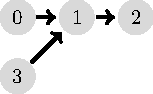
\includegraphics{figure1}}	
	\qquad
  \subfigure{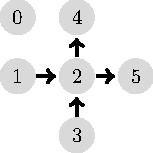
\includegraphics{figure2}}	
	\caption{Illustration of the Sample Inputs.}
\end{figure}

\section*{Input}

%The input starts with an integer~$T$ specifying the number of test cases that follow.
%Each test case consists of an integer~$N$ specifying the number of planets ($0<N<=1000$).
The input begins with an integer~$N$ specifying the number of planets ($0<N\le1000$). The planets are numbered from $0$ to $N-1$. The following $N$ lines specify the hyperspace connections. The $i$-th of those lines first contains the count of connections~$K$ ($0\le K\le N-1$) ~ \emph{from} planet~$i$ followed by $K$ integers specifying the destination planets.

\section*{Output}

%For each test case, output on a single line the minimum number of persons needed to visit every planet.
Output the minimum number of persons needed to visit every planet.
